% !TeX program = pdflatex


\documentclass[12pt]{article}
% for the equation* environment
\usepackage{amsmath}
\usepackage{amssymb}
\usepackage{amsthm}
\usepackage{amsfonts}

\usepackage{alphabeta}

\usepackage{csquotes}
\usepackage{subfigure}
\usepackage{float,lipsum}
\floatstyle{boxed}
\usepackage[top=3cm, bottom=3cm]{geometry}

\setlength{\footnotesep}{1.5em} % Adjust the value to set the desired distance

\usepackage{fullwidth}
\usepackage{float}	% avoid float repositioning
\usepackage{longtable}	% allow table to span multiple pages

% for images
\usepackage{graphicx}
\graphicspath{{images/}}

% to easily align image to left and right inside the includegraphics
% options
\usepackage[export]{adjustbox}
% and then \includegraphics[width=0.5\textwidth, right]{image}


% for captions
\usepackage{caption}

% for clickable table of contents entries
\usepackage{hyperref}

\hypersetup{
	colorlinks=false,
	linkcolor=black,
	filecolor=magenta,      
	urlcolor=blue,
	pdftitle={TheNegotiator}, % this is what appears as the title in the PDF viewer
	pdfpagemode=FullScreen,
}

% to number equations withing sections (1.1, 1.2, 2.1, and so on)
\numberwithin{equation}{section}

% to rename references to figures and such
\usepackage{cleveref}
\crefformat{figure}{fig.~#2#1#3}
\crefformat{table}{table~#2#1#3}


% to easily enclose text in quotes
\newcommand{\quotes}[1]{\textquotedblleft #1\textquotedblright \ }


\author{%
	Petros Bimpiris
	\and
	Ioannis Christofilogiannis
}

\date{
	\begin{center}
	\hspace{2.5cm}Technical University of Crete
	\newline
	\phantom{-----------------}Multiagent Systems (COMP512)		% what hack?
	\newline
	February 2024 
	\end{center}
	\vspace{-0.5cm}
}

\title{
	\vspace{-2cm}
	\textbf{TheNegotiator - Using Others To One's Advantage}

	Manipulation 101
}


\begin{document} 

	\maketitle

	\section*{Executive Summary}	\label{sec:execuctive_summary}		% non-technical and brief explanation - as if read by your grandma

		\paragraph*{}
			This report offers a comprehensive explanation and analysis of the design and the implementation of TheNegotiator agent. Its goal is to explain the basic ideas in a simple manner while simultaneously offering a detailed and robust technical description of the way they were implemented.
			% TODO: change the reference here to refer to the subsection of the intro that explains the rules
			The agent was designed to participate in an internal competition at Technical University of Crete, the basic concept of which was that pairs of agents engage in negotiation rounds repeatedly (so that all participants get to play each other) and the winner is declared based on the average \quotes{satisfaction} with the results achieved.
			The basic idea is that the TheNegotiator does not have a strategy of its own but incorporates an \quotes{arsenal} of other agents and has a way of picking the best one for each negotiation domain. The agent was heavily influenced \cite{meta_agent_paper} and its main idea that \quotes{\emph{a little learning goes a long way}}.	% 'domain' is overly technical here, need something like 'setting', 'round' or sth


	\section*{Report Structure}	\label{sec:report_structure}		% how this report is organized

		\paragraph*{}
			% better word for description here?
			The report begins with a description of the negotiation problem and the competition setting followed by an explanation of the basic ideas, the reasoning behind their adoption and some terminology definitions.
			We then proceed to the agent implementation, breaking it down to three parts: the way in which we use other agents as our strategy, the way of predicting each agent's performance in a new domain, and the way with which data collected during the competition can be used to further boost our performance. Finally we present and comment on various results that showcase strengths and limitations of our agent and we conclude by discussing possible steps towards improving on our ideas.
			\hfill

			Each section begins with a brief non-technical explanation of the concepts described therein and proceeds to explain them rigorously.

	\newpage

	\tableofcontents

	\newpage

	\section{Introduction}		\label{sec:introduction}

		\paragraph*{}
		In this section we describe the setting of negotiation 


		\subsection{The Negotiation Problem}	\label{sec:introduction.the_negotiation_problem}	% TODO: not problem, find a better word
			First things first: what \emph{exactly} do we mean by \quotes{negotiation}? Why would a computer ever need to do that? Even though we will not defend the existence of the academic field of negotiating agents, we will try to provide some motivation for our specific case.	% TODO: this sentence sucks but the meaning is nice, find a better way to say it


			\paragraph*{}

				The setting of a negotiation is best understood with the help of an example, so let us consider a scenario of two friends in a (peculiar) restaurant, where they must order the same thing, and they must order withing a time limit or they get no food. There are 2 issues: what to eat and what to drink. Possible values for the first issue are e.g. steak, salad or soup and for the second one beer or wine. The process is that one friend begins by proposing a value for each issue and then the other can either agree or extend a counteroffer. The goal is to reach an agreement and order before the waiter leaves.
			
			\paragraph*{}
				Some of the difficulties of a negotiation setting are apparent in the above example. What if the two friends have completely different tastes (i.e. preference profiles)? Should one agree to something that they do not like, just to avoid the scenario of the waiter leaving? - after all, food you don't like is better than no food at all. What if one friend only cares about food while the other only cares about drink? How are they supposed to find out - remember, they can only talk in terms of offers.
				Other difficulties are more subtle: What if there are 10 issues, with 20 possible values each? We then have $20^{10}$ different combinations (around 10.2 \emph{trillion}) - there is no way they can check them all before the waiter leaves. What if on top of that, each friend does not know the other's taste? Is an agreement even possible in such a scenario?

			\paragraph*{}
				The utilization of software agents for negotiations slowly starts to make a lot of sense. However, if we are to make a computer do all that, we need to be quite explicit. The following is a semi-formal definition of the concepts demonstrated in the restaurant example:

				\quad
				
				\renewcommand{\arraystretch}{1.5} % Adjust the value as needed
				\begin{longtable}{l p{290pt}}

						\textbf{Issues}: & The set $I$ of issues that the parties must agree upon values for. In the restaurant example, $I=\{\text{food}, \text{drink}\}$. \\

						\textbf{Values}: & The set $V$ of values for each issue in $I$. In the restaurant example, $V=$ $\{\{\text{steak}, \text{salad}, \text{soup}\}, \{\text{wine}, \text{beer}\}\}$.\\

						\textbf{Offer:} & An assignment $o$ of values to issues: $o=\{(i_{1}, v_{1}), (i_{2}, v_{2}), ...\}$, where $i_{j} \in I$ and $v_{j} \in V$. Also referred to as a \emph{bid}. \\

						\textbf{Utility Function:} & A function $u: O \to \mathbb{R}$ (where $O$ is the set of all offers). The utility function of a participant defines their preference profile, so these terms may be used interchangeably. In the restaurant example, suppose that one friend prefers beer to wine and is indifferent between all the food options. Then their utility function could look something like:
						\begin{equation*}
							\begin{aligned}
								& u_{1}((\text{food}: \textit{any}), (\text{drink}: \text{beer}))=1, \\
								& u_{1}((\text{food}: \textit{any}), (\text{drink}: \text{wine}))=0.5,
							\end{aligned}
						\end{equation*}
						with the exact values depending on how much they like each alternative.\\

						\textbf{Domain:} & A negotiation domain $d$ is defined as a triad $(I, V, P)$, where $I$ and $V$ are defined above and $P$ is the set of preference profiles of the domain\protect\footnotemark.\\
	
						\textbf{Negotiation Session:} & A negotiation session $s$ is a sequence of offers and counteroffers, that begins when each participant is informed of the domain and their preference profile and ends either with an agreement or when a timeout is reached. \\

						\textbf{Competition:} & A competition $C$ is defind as a pair $(A, D)$, where $A$ is the set of all agents participating in $C$ and $D$ is the set of all domains that will be used. Every pair of agents in $A$ plays in every domain in $D$. Also referred to as a tournament (though it most certainly is not one).\\	% TODO: better language

				\end{longtable}

				\footnotetext{The utility functions are given to the agents as part of the domain. The restaurant example equivalent would be someone telling you what your taste is when you enter. This might seem weird at first, but it is a way to force the agents to be able to handle every possible preference profile that we might need them to have - an agent that can only negotiate with a pre-designed preference profile would be of little use compared to one that can adapt its strategy to any given profile.}


		\subsection{Other Things}	\label{sec:introduction.other_things}
			Some other introductory things that we need to say about negotiations, agents and strategies.
			For example define strategy, define strategy agent, define protocol etyc.

	\section{Basic Ideas}		\label{sec:basic_ideas}

		\paragraph*{}
			The main idea behind TheNegotiator is that we have no explicit strategy to propose, evaluate and accept offers, but we rather employ a set of other, peer-designed agents and pretend that we are one of them in each round. % TODO: etsi opws to lew fainetai san na eimaste diaforetikoi se kathe round. mporoume na eimaste kai idioi omws. we need that to come across
			This shifts the problem that we have to solve from the bilateral negotiation one to the algorithm selection one: \quotes{Which algorithm out of a set of possible candidates is likely to perform best for a well-defined problem} \cite{original_alg_selection_paper_1975}. A great source of inspiration and a starting point for further research has been \cite{meta_agent_paper}, which also offers more background and theoretical insight into the algorithm selection problem in our setting.
			
		\paragraph*{}
			A key piece of insight here is \emph{when exactly are we asked to choose a strategy}: by competition rules we are allowed to change our strategy between negotiation sessions, but not during one.
			In other words, we are free to pick the best strategy for every negotiation session right before it begins, as long as we stick with it during the whole session.
		
		\paragraph*{}
			Much like \cite{meta_agent_paper}, we approach the problem from a machine learning (ML) standpoint, using ML techniques to perform two key actions:
			\begin{itemize}
				\item estimate the performance of the available strategies on a never-before-seen domain
				\item maintain and adjust that estimate throughout the competition, taking into consideration the results we get when using each strategy
			\end{itemize}

	\section{Implementation}		\label{sec:implementation}

		\subsection{High Level Overview}	\label{sec:implementation.high_level_view}

			\paragraph*{}
				The first step of the implementation was to pick our \quotes{\emph{arsenal}}, i.e. the set of readily available agents that we would use as our set of strategies. We used participants in the \href{https://web.tuat.ac.jp/~katfuji/ANAC2022/}{2022 ANAC competition} \cite{ANAC}, selected through a process described below. We chose to implement a neural network (NN), trained to find correlation between domain characteristics and agent performance to estimate how well those agents would do in a new domain. We also chose to model the competition as a Multi-Armed Bandit (MAB) % TODO: citation for MAB? where was it first defined?
				setting and implement a modified version of the Upper Confidence Bound (UCB) algorithm to keep learning during the competition while keeping performance as our primary objective.

			% picture here
			\begin{figure}[h]
				\centering
				\framebox{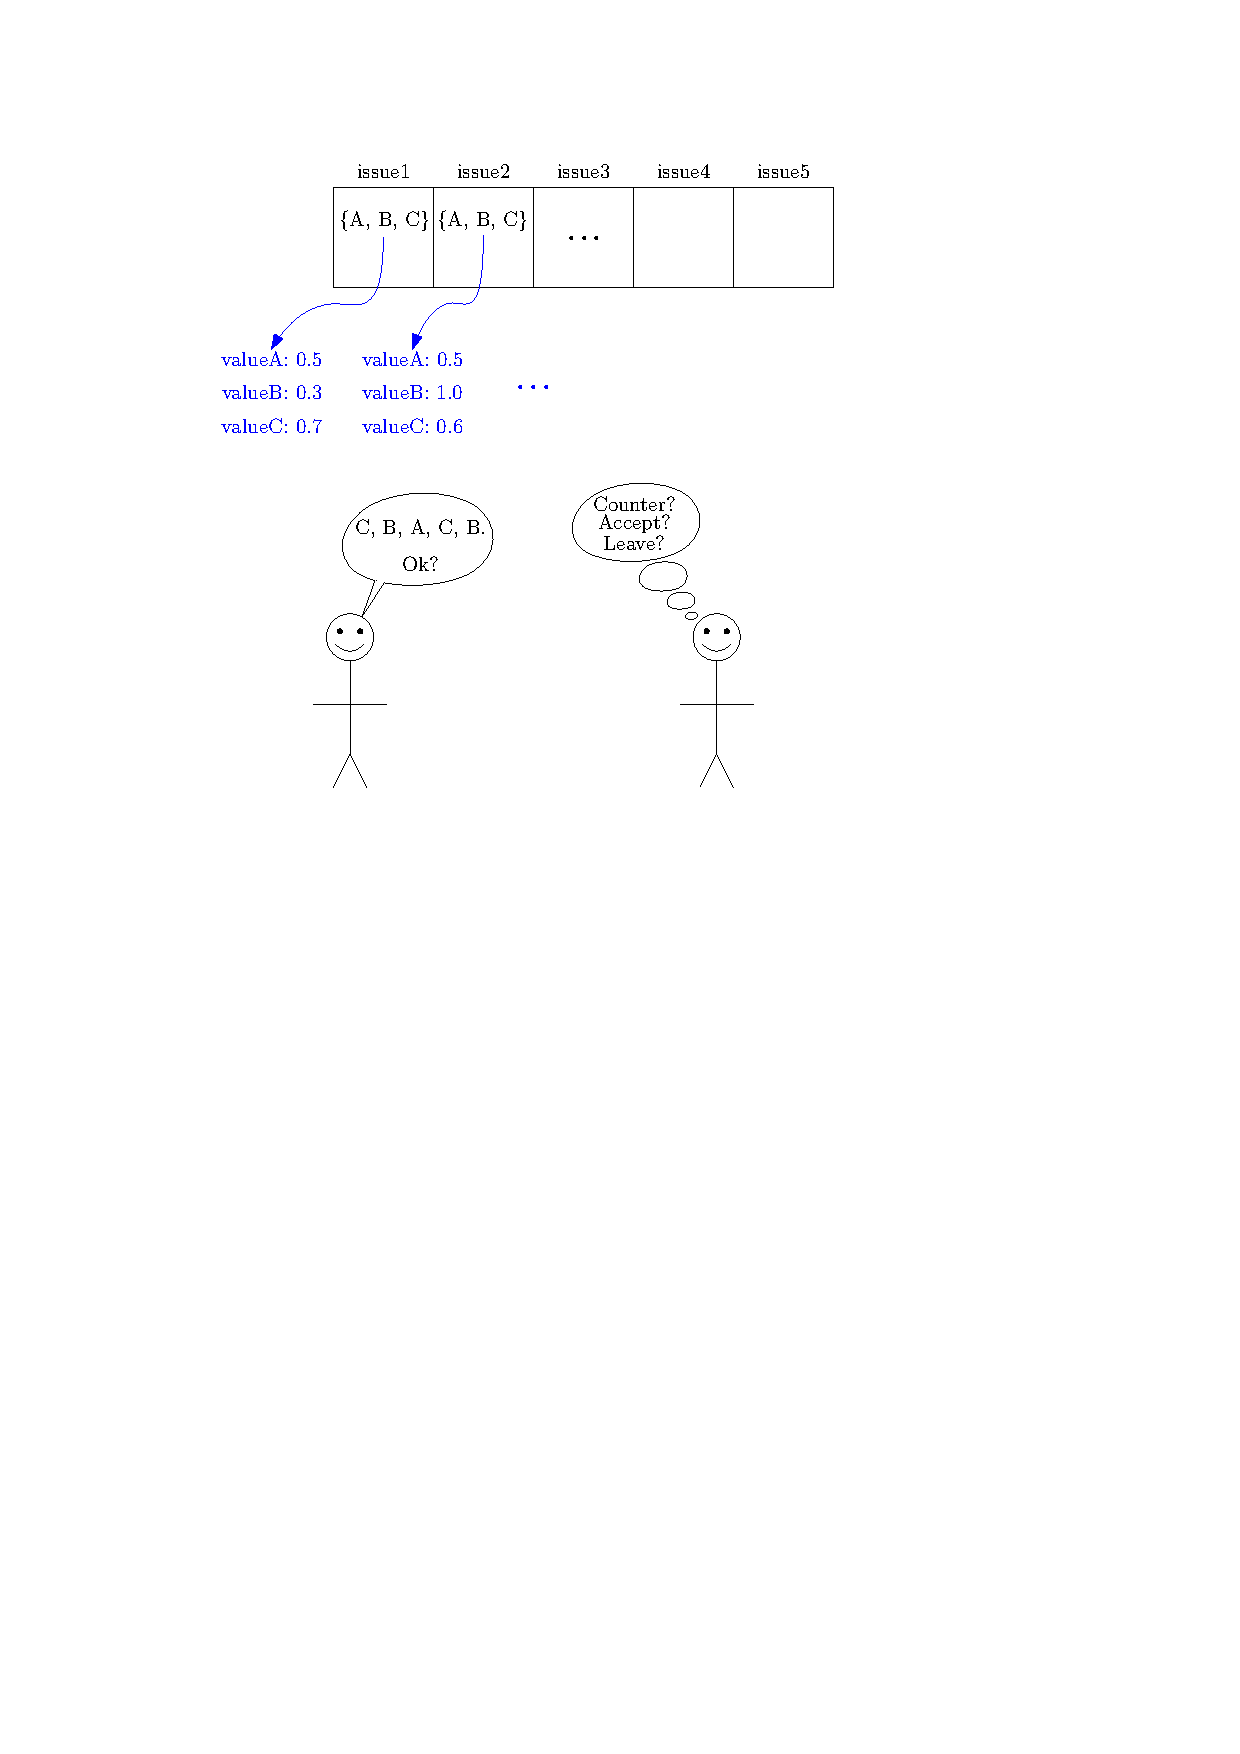
\includegraphics[scale=0.5]{issues_values.pdf}}
				\captionsetup{justification=centering}
				\caption{test figure}
				\label{fig:test_figure}
			\end{figure}



		\subsection{Using Other Agents}		\label{sec:implementation.using_other_agents}
			
			\paragraph{}


		
		\paragraph{}
A different strategy might perform better in one domain and worse in another.
Our goal was to find the correlation of the domain characteristics with the performance of each of the agents in our arsenal in that domain, in order to choose the one that will theoretically give us the best utility. 

\paragraph{}
 First we needed to collect data that will give us insight about the performance of each agent in a given domain. 
 This was handled by a custom runner, that ran negotiation rounds and stored the utility in files.
 \paragraph{}
 We set a negotiation setting with 5 agents in the arsenal, 10 opponents and 45 domains, meaning approximately 4500 negotiation rounds and approximately
10 hours of runtime (split into multiple computers by running the negotiations in separate domains in the same time).
\paragraph{}
 From this data we collected the average utility (the negotiation rounds with 10 opponents ) of each of the 5 agents and the characteristics of the domain. 
 The characteristics of the domain that we used are:
\begin{itemize}
	\item {Average bid utility} 
	\item {Average number of values per issue}
	\item {Bid utility standard deviation}
	\item {Number of bids}
	\item {Number of issues}
	\item {Weight Standard Deviation}
  
\end{itemize}

\paragraph{}
 The next logical step in order to handle this data is to use Machine Learning. Multiple viable methods exist 
 like CART which was the algorithm of choice for the Research Paper, along with others like Regression methods and a Neural Network , 
 but we decided to use a Neural Network (albeit with a different architecture) , because we were confident that this would be an effective, simple and efficient approach. 
 \paragraph{}
 In our problem the Neural Network 
 is a scalable solution because if the dataset becomes bigger, with more negotiation rounds, 
 the training time scales up, but we do not need to “carry” a huge dataset or retrain the model from scratch each time new data comes in, 
  neither is the structure itself growing in disk size. All we need to do is a training step for the new data, which consists of a forward pass with backpropagation.
\begin{figure}[H]
\centering
% First picture
\framebox{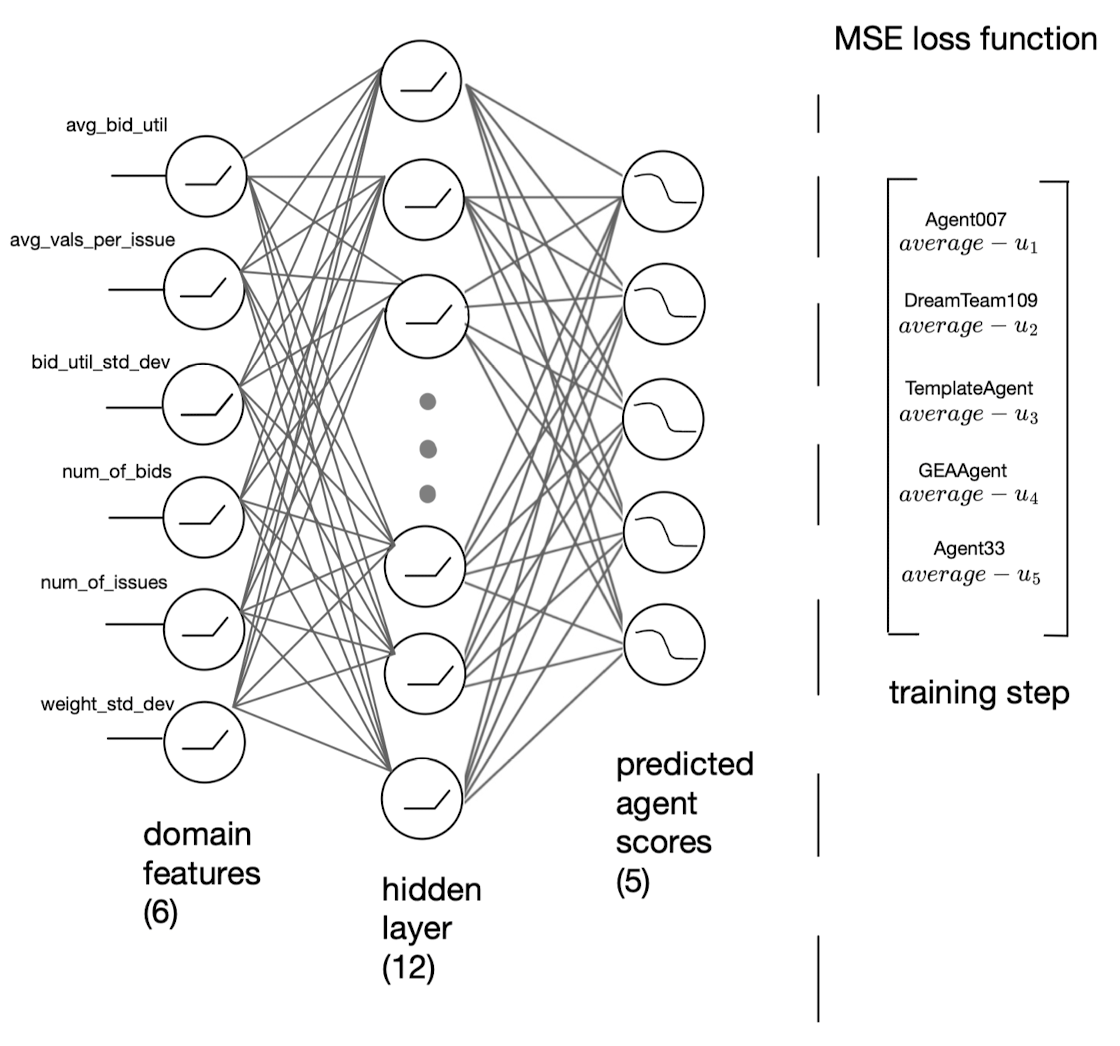
\includegraphics[scale=0.45]{nn_train.png}}
\captionsetup{justification=centering}
\caption{Neural Network Training}
\label{fig:NeuralNetworkTraining}
\end{figure}


\paragraph{}
 The Neural Network takes the domain characteristics (X) as input data along with the real average utility that the agents gained (Y) from the negotiation rounds in the specific domain. It’s goal is to train the Network (adjusting the weights and biases) so that giving the characteristics of a new domain gives us a prediction of each agent’s performance in it which can be very beneficial.  
 The training happens by passing the domain characteristics in a forwards pass, getting the outputs and using the Mean Square Error loss function to calculate the error between the outputs and the real scores and then using the optimizer, adam in our case to adjust the weights and biases with backpropagation.
 \paragraph{}
 

The architecture of the Neural Network is simple but a bit more complicated than the one decribed in the research paper \cite{meta_agent_paper}, even though not a lot of data is disclosed about it.
 We use an input layer of size 6, for each one of the domains characteristics, 
 a hidden layer of size 12 which is 2 times the size of input layer, in order to be able to detect hidden patterns in the data but showed 
 the best results between the values we tested and an output layer of size 5, for each of the agent's performance.  
 The input and hidden layers used the relu activation function and the output layer used the softmax activation function, which ensures that the outputs are a value between 0 and 1 and is a good fit for our predictions problem. We used 2 epochs for the training because it showed good results with no overfitting, like 3 or more epochs (showing similar results for different input features) and
  more effective training rounds than 1 epoch. Finally a dropout layer was applied (not shown in the figure, between the hidden layer and the output) with a dropout chance of 30\% that works by 
  randomly setting a fraction of input units to 0 at each update during training, which helps to make the model more robust and generalize better to unseen data. 
\paragraph{}



After the training is done to get the predictions for each agents, 
all we need is a forward pass of the domain characteristics from the Neural Network. 
This concludes the off-line training part of the problem, but the scope of the Negotiator does not stop there.
In the next part we test how the output of the Neural Network can give some knowledge to an on-line algorithm 
which will continue the learning with a different approach.
\begin{figure}[H]
	\centering
	\framebox{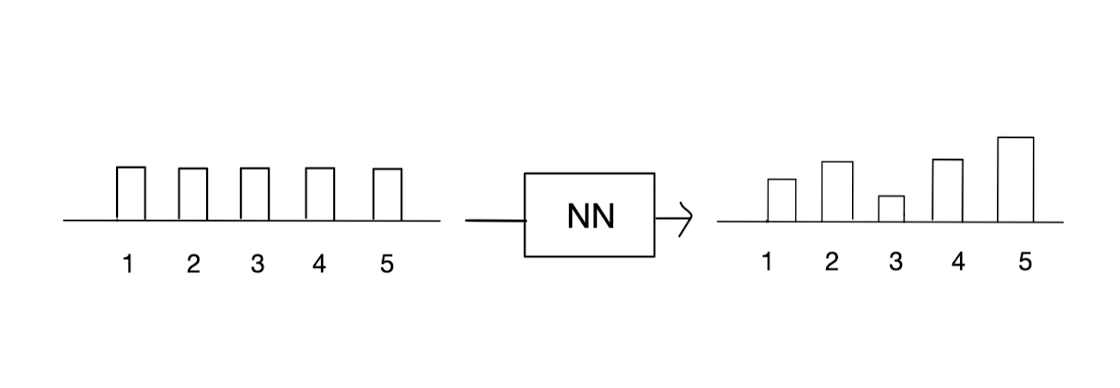
\includegraphics[scale=0.55]{nn_ucb.png}}
	\captionsetup{justification=centering}
	\caption{Setting the initial confidence bounds}
	\label{fig:Setting the initial confidence bounds}
\end{figure}
 
		
		\subsection{Online Learning - UCB}		\label{sec:implementation.ucb}

	\section{Results}		\label{sec:results}	% edw tha mporousan na paiksoun kai ta logs kalo rolo

	\section{Limitations \& Improvement Proposals}		\label{sec:limitations_improvements}

	\section{Conclusion}		\label{sec:conclusion}


	\bibliographystyle{plain}
	\bibliography{refs}


\end{document}